% !TEX encoding = UTF-8 Unicode
\documentclass[a4paper]{article}
\usepackage{titling}
\usepackage{makecell}
\usepackage{color}
\usepackage{float}
\usepackage{graphicx}
\usepackage{hyperref}
\usepackage{usecases}
\usepackage[utf8]{inputenc}
\usepackage[english,serbian]{babel}
\usepackage{listings}

\graphicspath{{./images/}}

\begin{document}

\title{Informacioni sistem poljoprivredne zadruge \small{Seminarski rad u okviru kursa\\Informacioni sistemi\\ Matematički fakultet}}

\author{Gajić Zorana, zorana.gajic.zg@gmail.com, 1091/2019 \\ 
        Dimić Nikola, dimic.nikola@gmail.com, 1098/2019 \\
        Jakovljević Aleksandar, a.jakovljevic96@gmail.com, 1090/2019 \\ 
        Veljković Marko, marko.veljko@gmail.com, 1096/2019}

\date{Novembar 2019}

\maketitle

\newpage

\tableofcontents

\newpage

\section{Uvod}
\subsection{Analiza sistema}

Detaljnom analizom načina funkcionisanja zadruga kako u poljoprivredi tako i u usko srodnim oblastima, došlo se do zaključka da je za potrebe gore pomenutih preduzeća potreban stabilan, efektivan i dobro projektovan informacioni sistem. Ovaj informacioni sistem doprineo bi kako članovima poljoprivrednih zadruga, tako i potencijalnim kupcima poljoprivrednih dobara. Kao glavni zahtevi i problemi prepoznate su sledeće stavke:

\begin{itemize}
  \item \textit{Jednostavan pristup} - Potrebno je da svi potencijalni članovi zadruge mogu lako pristupiti zadruzi i da se o članovima zadruge odlučuje na demokratski način, odnosno da postojeći članovi imaju uvid u proces pristupanja novih članova zadruge. Sistem kao i cela procedura mora funkcionisati brzo kako bi se potencijalni članovi motivisali da koriste informacioni sistem. 
  
  \item \textit{Kupovina i prodaja} - Potrebno je omogućiti laku potražnju za proizvodima, omogućiti članovima da svoje proizvode prodaju jednostavno a kupcima da imaju detaljan uvid u stanje poljoprivrednih dobara za koje su zainteresovani.
  
  \item \textit{Transparentnost} - Potrebno je da finansije unutar zadruge budu transparentne, kao i da svaka operacija koja uključuje potrošnju zajedničkih dobara bude odobrena od strane većinskog dela članova zadruge. Prikupljanje dobrovoljnih priloga kao i redovne članarine treba da bude bezbedno i jednostavno. 
\end{itemize}


\subsection{Akteri}
\indent  Akteri ovog informacionog sistema predstavljeni su i kasnije referisani na sledeći način:


\subsubsection{Član zadruge}
\indent Član zadruge ima sledeće mogućnosti korišćenja sistema:
\begin{itemize}
    \item Glasa prilikom donošenja odluka zadruge (svaki glas ima podjednaku važnost)
    \item Unosi nove predloge u sistem koji se potom šalju na glasanje
    \item Ima mogućnost potraživanja sredstava i mašina potrebnih za proizvodnju
    \item Ima mogućnost obezbeđivanja sredstava i mašina u svrhu korišćenja drugih zadrugara
    \item Može istupiti iz zadruge, ukoliko nema nikakva dugovanja prema istoj
    \item Plaća mesečnu članarinu ili daje dobrotvorni prilog
    
\end{itemize}

\subsubsection{Kupac}
\indent Kupac ima sledeće mogućnosti korišćenja sistema:
\begin{itemize}
    \item Naručuje proizvode koji se nalaze na sajtu
    \item Plaća naručene proizvode i dostavlja potvrdu
    \item Šalje predloge koji bi proizvodi mogli da se nađu u ponudi
\end{itemize}

\subsubsection{Kooperant (proizvođač)}
\indent Kooperant ima sledeće mogućnosti korišćenja sistema:
\begin{itemize}
    \item Dobija narudžbinu i rok do kada mora dostaviti proizvod
    \item Odgovara na dobijenu narudžbinu i prosleđuje traženu cenu
    \item Dobija odgovor o ceni (potvrda/otkazivanje) porudžbine
    \item Obaveštava zadrugu o završenoj proizvodnji
    \item Ima mogucnost slanja zahteva za učlanjenje u zadrugu
\end{itemize}

\subsubsection{Direktor}
\indent Direktor ima sledeće mogućnosti korišćenja sistema:
\begin{itemize}
    \item Prihvata ili odbacuje zahtev za primanje novog člana
    \item Izbacuje člana iz zadruge
    \item Šalje zahtev za skladištenje i/ili preradu proizvoda
    \item Predlaže potražnju mašine ili sredstva za zadrugu
    \item Odobrava korišćenje sredstava zadruge
\end{itemize}

%\subsubsection{Administrator}
%\indent Ima sledeće mogućnosti korišćenja sistema:
%\begin{itemize}
%    \item Dodaje nove članove u sistem
%    \item Menja uloge članova sistema po potrebi (unapređuje i unazađuje)
%    \item Izbacuje članove iz sistema
%\end{itemize}

\subsubsection{Blagajnik}
\indent Ima sledeće mogućnosti korišćenja sistema:
\begin{itemize}
    \item Ima uvid u dugovanja svih članova zadruge
    \item Koristi sredstva zadruge za javne nabavke
    \item Ima uvid u odluke članova zadruge o potrošnji zajedničkih dobara
\end{itemize}

\subsubsection{Neregistrovani korisnik}
\indent Ima sledeće mogućnosti korišćenja sistema:
\begin{itemize}
    \item Registruje svoj nalog
\end{itemize}

\newpage

\section{Slučajevi upotrebe}
Na slici \ref{dtp_nivo_0} je prikazan dijagram konteksta kao i akteri.
\begin{figure}[h!]
    \centering
    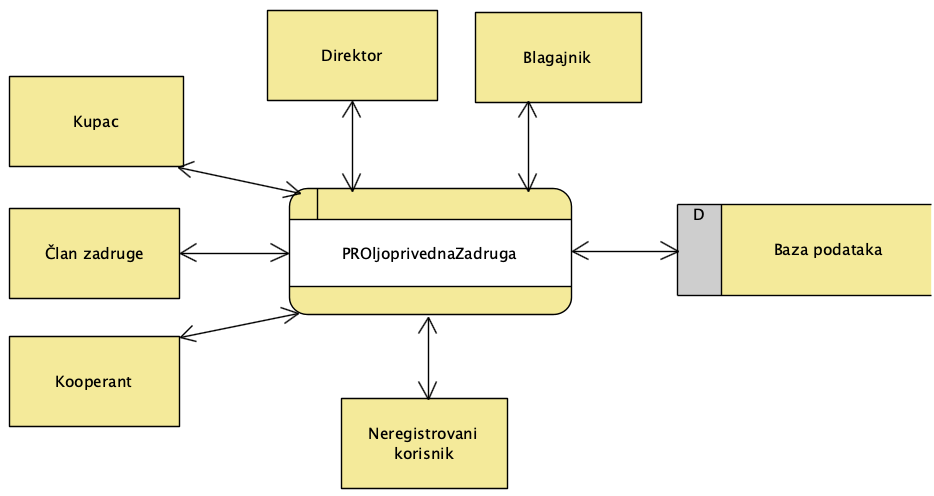
\includegraphics[scale=0.72]{images/dtp_nivo_0.png}
    \caption{Dijagram konteksta}
    \label{dtp_nivo_0}
\end{figure}


\subsection{Nalozi}

\begin{figure}[h!]
    \centering
    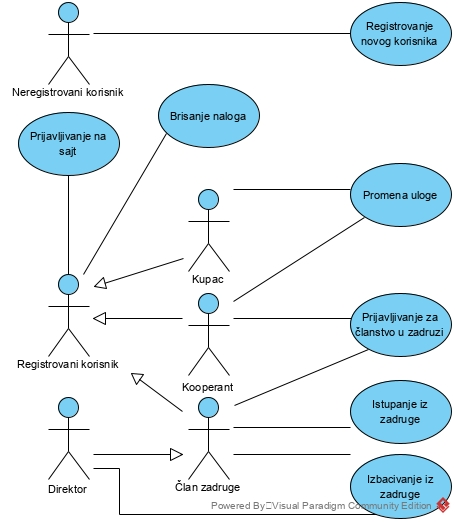
\includegraphics[scale=0.65]{images/clanstvoSU.jpg}
    \caption{Dijagram slučajeva upotrebe vezanih za vrste naloga u sistemu}
    \label{slika1}
\end{figure}

\subsubsection{Registrovanje korisnika}
\begin{usecase}
        \addtitle{SLUČAJ UPOTREBE}{}
        \addfield{Naziv:}{Registracija novog korisnika}
        \addfield{Kratak opis:}{Neregistrovan korisnik želi da napravi svoj nalog}
        \addfield{Učesnici:}{
            Neregistrovani korisnik 
        }
        \addfield{Preduslovi:}{
            Email adresa korisnika ne postoji u sistemu
        }
        \addfield{Postuslovi:}{
            Korisnik je uspešno registrovan u sistemu i baza podataka je ažurirana
        }

        \addscenario{Glavni tok:}{
            \item Korisnik odlazi na vebsajt i otvara formu za registraciju
            \item Korisnik popunjava formu za registraciju
            \item Korisnik bira ulogu kooperanta
            \item Korisnik popunjava dodatna polja koja se prikazuju samo budućem kooperantu 
            \item Korisnik potvrđuje svoju registraciju
            \item Sistem vrši validaciju registracije
            \item Sistem pamti unetu registraciju
            \item Sistem obaveštava korisnika o uspešnoj registraciji
        }
        \addscenario{Alternativni tokovi:}{
            \item[3.a] Ukoliko je korisnik izabrao ulogu kupca, slučaj upotrebe se nastavlja od koraka 5.
            \item[6.a] Ukoliko je korisnik odabrao korisničko ime koje već postoji u sistemu, prikazuje se odgovarajuća poruka. Slučaj upotrebe se nastavlja od koraka 2.
            \item[6.b] Ukoliko je korisnik odabrao lozinku koja ne odgovara specifikacijama sistema (prekratka, nema nijedan broj, nema nijedno veliko slovo), prikazuje se odgovarajuća poruka. Slučaj upotrebe se nastavlja od koraka 2.
            \item[6.c] Ukoliko korisnik nije popunio sva polja forme, prikazuje se odgovarajuća poruka. Slučaj upotrebe se nastavlja od koraka 2.
            \item[6.d] Ukoliko korisnik nije izabrao ulogu koju želi da ima u sistemu, prikazuje se odgovarajuća poruka. Slučaj upotrebe se nastavlja od koraka 3.
            \item[6.e] Ukoliko korisnik nije popunio odgovarajuća polja vezana za kooperanta, prikazuje se odgovarajuća poruka. Slučaj upotrebe se nastavlja od koraka 4.
            \item[6.f] Ukoliko korisnik nije popunio odgovarajuća polja vezana za karticu, prikazuje se odgovarajuća poruka. Slučaj upotrebe se nastavlja od koraka 4.
        }
        
        \addfield{Dodatne informacije:}{Forma za prijavu sadrži sledeća polja: korisničko ime, lozinku, email adresu, broj telefona, izbor uloge u okviru sistema (kupac/kooperant) i podatke sa kartice (kreditna/debitna). Dodatna polja koja popunjava korisnik koji je izabrao ulogu kooperanta su: predmet proizvodnje, mesto proizvodnje, količina proizvoda, cena porizvoda.
        }
\end{usecase}

\newpage
\subsubsection{Prijavljivanje na sajt}
\begin{usecase}
        \addtitle{SLUČAJ UPOTREBE}{}
        \addfield{Naziv:}{Prijavljivanje korisnika}
        \addfield{Kratak opis:}{Prijavljivanje već postojećeg korisnika}
        \addfield{Učesnici:}{
            Registrovani korisnik (član zadruge/kooperant/kupac) 
        }
        \addfield{Preduslovi:}{
            Korisnik je prethodno registrovan
        }
        \addfield{Postuslovi:}{
            Korisnik je uspešno pristupio svom nalogu
        }

        \addscenario{Glavni tok:}{
            \item Korisnik odlazi na vebsajt i otvara formu za prijavu
            \item Korisnik unosi korisničko ime i lozinku
            \item Korisnik potvrđuje svoj unos
            \item Sistem vrši validaciju prijave
            \item Korisnik je prijavljen na svoj nalog
        }
        \addscenario{Alternativni tokovi:}{
            \item[4.a] Ukoliko je korisnik uneo nepostojeće korisničko ime, prikazuje se odgovarajuća poruka. Slučaj upotrebe se nastavlja od koraka 2.
            \item[4.b] Ukoliko je korisnik uneo neispravnu lozinku, prikazuje se odgovarajuća poruka. Slučaj upotrebe se nastavlja od koraka 2.
        }
\end{usecase}


\subsubsection{Apliciranje za članstvo}
\begin{usecase}
        \addtitle{SLUČAJ UPOTREBE}{}
        \addfield{Naziv:}{Apliciranje za članstvo u zadruzi}
        \addfield{Kratak opis:}{Kooperant, odnosno korisnik koji je registrovan u sistemu kao proizvođač šalje zahtev za učlanjivanje u zadrugu}
        \addfield{Učesnici:}{
             Kooperant, članovi zadruge
        }
        \addfield{Preduslovi:}{
            Korisnik je registrovan u sistemu kao kooperant 
        }
        \addfield{Postuslovi:}{
            Kooperant je dobio odgovor na svoj zahtev i ukoliko je potvrdan, postao je ravnopravni član zadruge
        }

        \addscenario{Glavni tok:}{
            \item Korisnik odlazi na vebsajt i prijavljuje se
            \item Korisnik popunjava podatke neophodne za apliciranje za članstvo u zadruzi
            \item Korisnik šalje zahtev na obradu
            \item Sistem vrši validaciju prijave
            \item Sistem prihvata zahtev za članstvo i prosleđuje ga članovima zadruge 
            \item Članovi zadruge imaju rok od 72h da izvrše glasanje za prihvatanje novog člana
            \item Korisnik se obaveštava da je primljen u zadrugu
            \item Uloga trenutnog korisnika je promenjena u sistemu i on je sada ravnopravni član zadruge 
        }
        \addscenario{Alternativni tokovi:}{
            \item[4.a] Ukoliko korisnik nije uneo sve potrebne podatke i/ili podaci nisu u traženom formatu, prikazuje se odgovarajuća poruka. Slučaj upotrebe se nastavlja od koraka 2.
            \item[7.a] Ukoliko korisnik nije primljen u zadrugu, ostaje kooperant i može se ponovo prijaviti za nedelju dana. Slučaj upotrebe se završava.
        }
        \addfield{Dodatne informacije:}{
            Informacije koje korisnik unosi u zahtevu za članstvo su: razlog za pristupanje zadruzi, vremenski period u ulozi kooperanta zadruge, proizvodi prodavani zadruzi, dodatni proizvodi koje bi mogao da prodaje, način doprinosa zadruzi.
        }
\end{usecase}


\subsubsection{Istupanje iz zadruge}
\begin{usecase}
        \addtitle{SLUČAJ UPOTREBE}{}
        \addfield{Naziv:}{Istupanje iz zadruge}
        \addfield{Kratak opis:}{Član zadruge želi da istupi iz iste uz mogućnost odabira svoje uloge u sistemu kooperant/kupac/potpuno brisanje naloga}
        \addfield{Učesnici:}{
             Član zadruge
        }
        \addfield{Preduslovi:}{
           Korisnik je član zadruge
        }
        \addfield{Postuslovi:}{
           Korisnik više nije član zadruge
        }

        \addscenario{Glavni tok:}{
            \item Korisnik odlazi na vebsajt i prijavljuje se
            \item Korisnik odabira opciju napuštanja zadruge 
            \item Korisnik unosi razlog za napuštanje zadruge 
            \item Korisnik odabira brisanje naloga kao novu ulogu unutar sistema
            \item Korisnik šalje popunjeni zahtev 
            \item Sistem obrađuje zahtev 
            \item Menja se uloga korisnika u bazi podataka
            \item Korisnik dobija poruku o uspešnom napuštanju zadruge
        }
        \addscenario{Alternativni tokovi:}{
            \item[4.a] Ukoliko je korisnik izabrao da postane kooperant, sistem obrađuje zahtev i obaveštava zadrugara da od sada ima ulogu kooperanta. Slučaj upotrebe se završava.
            \item[4.b] Ukoliko je korisnik izabrao da postane kupac, sistem obrađuje zahtev i obaveštava korisnika da od sada ima ulogu kupca. Slučaj upotrebe se završava.
            \item[5.a] Ukoliko je korisnik ipak rešio da ostane član (napuštanjem forme ili poništavanjem unetih podataka), slučaj upotrebe se završava.
    
        }
\end{usecase}

\subsubsection{Izbacivanje iz zadruge}
\begin{usecase}
        \addtitle{SLUČAJ UPOTREBE}{}
        \addfield{Naziv:}{Izbacivanje člana iz zadruge}
        \addfield{Kratak opis:}{Član zadruge je prekršio neko od osnovnih pravila i direktor zadruge je rešio da ga izbaci iz iste}
        \addfield{Učesnici:}{
            Član zadruge, direktor
        }
        \addfield{Preduslovi:}{
           Korisnik je član zadruge i prekršio je neko od osnovnih pravila
        }
        \addfield{Postuslovi:}{
           Korisnik više nije član zadruge i ne može se prijaviti za u istu u narednih godinu dana
        }

        \addscenario{Glavni tok:}{
            \item Direktor zadruge odlazi na vebsajt i prijavljuje se
            \item Direktor pronalazi odgovarajućeg korisnika u sistemu i prelazi na formu za izbacivanje člana iz zadruge
            \item Direktor unosi razlog ga izbacivanje člana iz zadruge, odnosno bira koje je pravilo prekršio član zadruge
            \item Direktor potvrđuje unesene podatke
            \item Sistem obrađuje zahtev
            \item Član zadruge je izbrisan iz sistema
            \item Korisnik dobija automatsku poruku na email adresu koja sadrži razlog izbacivanja i obaveštenje da je njegov nalog izbrisan
        }
        \addscenario{Alternativni tokovi:}{
            \item[4.a] Ukoliko je direktor ipak rešio da ne izbaci člana iz zadruge (napuštanjem forme ili poništavanjem unetih podataka), slučaj upotrebe se završava.
        }
\end{usecase}


\subsubsection{Promena uloge}
\begin{usecase}
        \addtitle{SLUČAJ UPOTREBE}{}
        \addfield{Naziv:}{Promena uloge korisnika sistema}
        \addfield{Kratak opis:}{Korisnik koji ima ulogu kupca/kooperanta želi da postane kooperant/kupac}
        \addfield{Učesnici:}{
            Kooperant, kupac
        }
        \addfield{Preduslovi:}{
           Korisnik je registrovan u sistemu i nije član zadruge
        }
        \addfield{Postuslovi:}{
           Uloga korisnika u sistemu je uspešno promenjena i baza podataka je ažurirana
        }

        \addscenario{Glavni tok:}{
            \item Korisnik odlazi na vebsajt i prijavljuje se
            \item Korisnik prelazi na formu za promenu uloge
            \item Korisnik unosi razlog za promenu uloge 
            \item Korisnik je trenutno kupac i izabrao je da želi postati kooperant
            \item Korisnik popunjava preostala dodatna polja
            \item Korisnik potvrđuje unesene podatke
            \item Sistem obrađuje zahtev
            \item Uloga korisnika je uspešno promenjena u sistemu
        }
        \addscenario{Alternativni tokovi:}{
            \item[4.a] Ukoliko je korisnik trenutno kooperant i izabrao je da postane kupac. Slučaj upotrebe se nastavlja od koraka 5.
            \item[7.a] Ukoliko korisnik nije popunio dodatna polja, prikazuje se obaveštenje sa informacijom koja su polja obavezna. Slučaj upotrebe se nastavlja od koraka 5.
        }
        \addfield{Dodatne informacije:}{
           Dodatna polja koja popunjava kupac koji želi postati kooperant: predmet proizvodnje, mesto proizvodnje, količina proizvodnje, cena proizvoda.
        }
\end{usecase}

\subsubsection{Brisanje naloga}
\begin{usecase}
        \addtitle{SLUČAJ UPOTREBE}{}
        \addfield{Naziv:}{Brisanje naloga iz sistema}
        \addfield{Kratak opis:}{Korisnik želi da obriše svoj nalog}
        \addfield{Učesnici:}{
            Registrovani korisnik (član zadruge/kooperant/kupac)
        }
        \addfield{Preduslovi:}{
           Korisnik je registrovan u sistemu
        }
        \addfield{Postuslovi:}{
           Nalog korisnika je uspešno obrisan i njegova email adresa je izbrisana iz baze podataka
        }

        \addscenario{Glavni tok:}{
            \item Korisnik odlazi na vebsajt i prijavljuje se
            \item Korisnik prelazi na formu za brisanje naloga
            \item Korisnik unosi razlog brisanja naloga
            \item Korisnik potvrđuje unesene podatke 
            \item Korisnik šalje zahtev sistemu
            \item Sistem obrađuje zahtev
            \item Nalog korisnika je uspešno obrisan iz sistema
        }
        \addscenario{Alternativni tokovi:}{
            \item[2.a] Trenutni korisnik je član zadruge. Dobija poruku da se prvo mora isčlaniti iz zadruge i biva preusmeren na slučaj upotrebe \hyperref[subsubsec:istupanjeIzZadruge]{'Istupanje iz zadruge'}. Slučaj upotrebe se završava.
            \item[4.a] Ukoliko je korisnik ipak rešio da ne obriše nalog (napuštanjem forme ili poništavanjem unetih podataka), slučaj upotrebe se završava.
        }
\end{usecase}


\subsection{Proizvodnja}

Neke beleske sa dogovora (dodaću sutra neke od ovih slučajeva): 
\begin{itemize}
  \item Slanje zahteva za proizvodnjom - clan salje clanu/koooperatoru (ovo moramo jos da vidimo kako cemo nije bas najjasnije

  \item Potraivanje materijala i mašina - clan potrazuje drugom clanu mašinu ili pomoć
  
  \item Javljanje za materijal ili masinu da das drugome  ( + alternativa za sladiste) - odgovor na potrazivanje - popunis neke forme
  
  \item Slanje zahteva za skladištenjem - ovo je 2 kao alternativni put da umesto masine pozajmis skladiste)
  clan zahteva clanu da mu on skladisti u svom skladistu 
  
  \item Slanje ponude za prodaju
   clan salje svima(sistemu kupcima s....) sta ima na stanju 

  \item Plaćanje proizvodjacu, Slanje zahteva za preradu
  
  \item predlog kupovine eksternih dobara - direktor predlaze kupovinu (masina/materijala/...) za koriscenje zadruge iz budzeta - clanovi zadruge glasaju 
  
\end{itemize}



\subsubsection{Slanje zahteva za proizvodnjom}
\subsubsection{Potraživanje materijala i mašina}
\subsubsection{Slanje zahteva za skladištenjem}
\subsubsection{Slanje zahteva za preradu}
\subsubsection{Slanje ponude za prodaju}
\subsubsection{Plaćanje proizvođaču}

\subsection{Prodaja}
\subsubsection{Naručivanje proizvoda preko interneta}
\subsubsection{Naručivanje proizvoda preko telefona}
\subsubsection{Naručivanje proizvoda uživo u zadruzi}
\subsubsection{Dostavljanje potvrde o plaćanju}
\subsubsection{Organizacija dostave proizvoda}
\subsection{Ostalo}
\subsubsection{Davanje novčanog priloga}
\begin{usecase}
        \addtitle{SLUČAJ UPOTREBE}{}
        \addfield{Naziv:}{Davanje priloga}
        \addfield{Kratak opis:}{Registrovani korisnik želi da donira novac zadruzi}
        \addfield{Učesnici:}{
            Registrovani korisnik (član zadruge/kooperant/kupac)
        }
        \addfield{Preduslovi:}{
           Korisnik je registrovan u sistemu
        }
        \addfield{Postuslovi:}{
           Korisnik je izvršio novčanu donaciju ukoliko je sistem adekvatno obradio podatke
        }

        \addscenario{Glavni tok:}{
            \item Korisnik odlazi na vebsajt i prijavljuje se
            \item Korisnik prelazi na formu za doniranje novca
            \item Korisnik unosi količinu novca i svrhu donacije
            \item Korisnik potvrđuje unesene podatke 
            \item Korisnik šalje zahtev sistemu
            \item Sistem obrađuje zahtev
            \item Sistem ažurira stanje na računu
            \item Korisnik dobija potvrdu o uplati
        }         
        \addscenario{Alternativni tokovi:}{
            \item[4.a]  Ukoliko korisnik nije uneo količinu novca, svrhu ili je uneo pogrešan format, prikazuje se odgovarajuča poruka. Slučaj upotrebe se nastavlja od koraka 2.
            \item[6.a] Ukoliko uplata nije prošla, korisnik dobija opciju da se vrati na korak 2, inače slučaj upotrebe se završava.
        }
\end{usecase}
\subsubsection{Plaćanje mesečne članarine}
\begin{usecase}
        \addtitle{SLUČAJ UPOTREBE}{}
        \addfield{Naziv:}{Plaćanje mesečne članarine}
        \addfield{Kratak opis:}{Član zadruge želi da uplati mesečnu članarinu}
        \addfield{Učesnici:}{
            Član zadruge
        }
        \addfield{Preduslovi:}{
           Član zadruge je registrovan u sistemu
        }
        \addfield{Postuslovi:}{
           Član zadruge je platio članarinu ukoliko je sistem adekvatno obradio podatke
        }

        %Main Success Scenario: A typical, unconditional happy path scenario of success.
        \addscenario{Glavni tok:}{
            \item Korisnik odlazi na vebsajt i prijavljuje se
            \item Korisnik prelazi na formu za uplatu članarine
            \item Korisnik unosi vrednost članarine
            \item Korisnik potvrđuje unesene podatke
            \item Korisnik šalje zahtev sistemu
            \item Sistem obrađuje zahtev
            \item Sistem ažurira korisnikova zaduženja
            \item Korisnik dobija potvrdu o uplati
        }
        \addscenario{Alternativni tokovi:}{
            \item[4.a] Ukoliko korisnik nije uneo količinu novca, svrhu ili je uneo pogrešan format, prikazuje se odgovarajuča poruka. Slučaj upotrebe se nastavlja od koraka 2.
            \item[6.a] Ukoliko uplata nije prošla, korisnik dobija opciju da se vrati na korak 2, inače slučaj upotrebe se završava.
        }
\end{usecase}

\subsubsection{Izdvajanje sredstava za dodatne troškove}
\begin{usecase}
        \addtitle{SLUČAJ UPOTREBE}{}
        \addfield{Naziv:}{Izdvajanje sredstava za dodatne troškove}
        \addfield{Kratak opis:}{Direktor zahteva novac od blagajnika za pokrivanje dodatnih troškova i obaveštava članove zadruge}
        \addfield{Učesnici:}{
            Direktor,
            blagajnik,
            član zadruge
        }
        \addfield{Preduslovi:}{
           Stanje na računu zadruge je pozitivno
        }
        \addfield{Postuslovi:}{
           Stanje na računu zadruge je pozitivno
        }

        %Main Success Scenario: A typical, unconditional happy path scenario of success.
        \addscenario{Glavni tok:}{
            \item Direktor zadruge odlazi na vebsajt i prijavljuje se
            \item Direktor prelazi na formu za stvaranje dodatnog troška
            \item Direktor unosi razlog i potrebnu količinu novca za pokrivanje troškova
            \item Direktor potvrđuje unesene podatke
            \item Direktor šalje zahtev blagajniku
            \item Blagajnik proverava zahtev direktora
            \item Blagajnik obaveštava direktora o statusu zahteva
            \item Blagajnik odvaja novac za dodatni trošak
            \item Blagajnik obaveštava direktora da je novac izdvojen
            \item Direktor obaveštava članove zadruge o dodatnim troškovima
        }
        \addscenario{Alternativni tokovi:}{
            \item[4.a] Ukoliko direktor nije uneo razlog za pokrivanje troškova, prikazuje se odgovarajuća poruka. Slučaj upotrebe se nastavlja od koraka 2.
            \item[4.b] Ukoliko direktor nije uneo potrebnu količinu novca za pokrivanje troškova, prikazuje se odgovarajuća poruka. Slučaj upotrebe se nastavlja od koraka 2.
            \item[7.a] Ukoliko bi stanje na računu postalo negativno nakon izdvajanja novca, blagajnik obaveštava direktora da nije moguće trenutno izdvojiti potrebnu količinu novca za pokrivanje troškova. Slučaj upotrebe se završava.
            
        }
\end{usecase}
\subsubsection{Izveštaj o potrošenim sredstvima}
\begin{usecase}
        \addtitle{SLUČAJ UPOTREBE}{}
        \addfield{Naziv:}{Izveštaj o potrošenim sredstvima}
        \addfield{Kratak opis:}{Blagajnik izveštava članove zadruge o utrošenom novcu}
        \addfield{Učesnici:}{
            Blagajnik, članovi zadruge
        }
        \addfield{Preduslovi:}{
           Svi učesnici su registrovani
        }
        \addfield{Postuslovi:}{
           Svi učesnici su obavešteni o tekučem stanju na računu zadruge i utrošenim sredstvima
        }

        %Main Success Scenario: A typical, unconditional happy path scenario of success.
        \addscenario{Glavni tok:}{
            \item Blagajnik zadruge odlazi na vebsaht i prijavljuje se
            \item Blagajnik prelazi na formu za stvaranje mesečnog izveštaja
            \item Blagajnik popunjava formu
            \item Blagajnik potvrđuje unesene podatke
            \item Sistem obrađuje zahtev
            \item Sistem generiše izveštaj
            \item Sistem obaveštava sve učesnike o tekućem stanju na računu zadruge
        }
        \addscenario{Alternativni tokovi:}{
            \item[4.a] Ukoliko blagajnik nije popunio formu, prikazuje se odgovarajuća poruka. Slučaj upotrebe se nastavlja od koraka 2.
            
        }
        \addfield{Dodatne informacije:}{Forma za stvaranje izveštaja sadrži sledeća polja: datum od kojeg se traže prihodi i rashodi, format dokumenta (pdf/docx/csv), korisnici kojima se šalje izveštaj (direktor/članovi zadruge)}
\end{usecase}

\section{Arhitektura sistema}

\section{Baza podataka}

\section{Korisnički interfejs}





% TEMPLATE ZA SLUCAJ UPOTREBE 
\subsubsection{}
\begin{usecase}
        \addtitle{SLUČAJ UPOTREBE}{}
        \addfield{Naziv:}{}
        \addfield{Kratak opis:}{}
        \addfield{Učesnici:}{
            
        }
        \addfield{Preduslovi:}{
           
        }
        \addfield{Postuslovi:}{
           
        }

        %Main Success Scenario: A typical, unconditional happy path scenario of success.
        \addscenario{Glavni tok:}{
            \item 
            
        }
        \addscenario{Alternativni tokovi:}{
            \item[2.a] 
            
        }
\end{usecase}
    
\end{document}
